\chapter{Related Work}
This chapter presents related work. The first section presents an article on the current state of research on MTD in IoT. The second section presents related work in the area of MTD frameworks for IoT devices. The last section gives an overview of specific IoT techniques and explains how they relate to the work at hand. 

\section{State of Research of MTD in IoT}
\cite{navas:2021MTDWhere} did a literature review analyzing existing MTD for IOT techniques. This section is based on that source. The authors defined four research questions, all of which are of interest in the context of this thesis. The first research question concerned the number of proposals for MTD techniques that exist for IoT. They concluded that since 2013, 32 novel proposals have been proposed for the IoT domain. In contrast, more than 80 different general purpose MTD techniques have been proposed from 2009 to 2018~\cite{website:surveyOfCyberMovingTargets}. 

The second research question was related to the characteristics that can be observed in MTD techniques for IoT. For this question, the authors created an MTD taxonomy showing the distribution of these 32 techniques grouped in the MTD domain mentioned in Section \ref{section:MTD}. The dominant techniques are the networking techniques with 54\%, followed by the dynamic runtime environment techniques with 20\%. Software and data techniques follow with 13\% and 10\%, respectively. Dynamic platform techniques have the smallest share with 3\%. Figure \ref{graphic:IoTShare} shows these shares graphically. These shares differ from those of the general-purpose MTD techniques, where, for example, the dynamic network techniques account for only about 21\% or the dynamic platform for about 20\%. A possible reason for this is that recently there has been an increasing interest in network-based MTD techniques~\cite{navas:2021MTDWhere}. 
 
 \begin{figure}[tph]
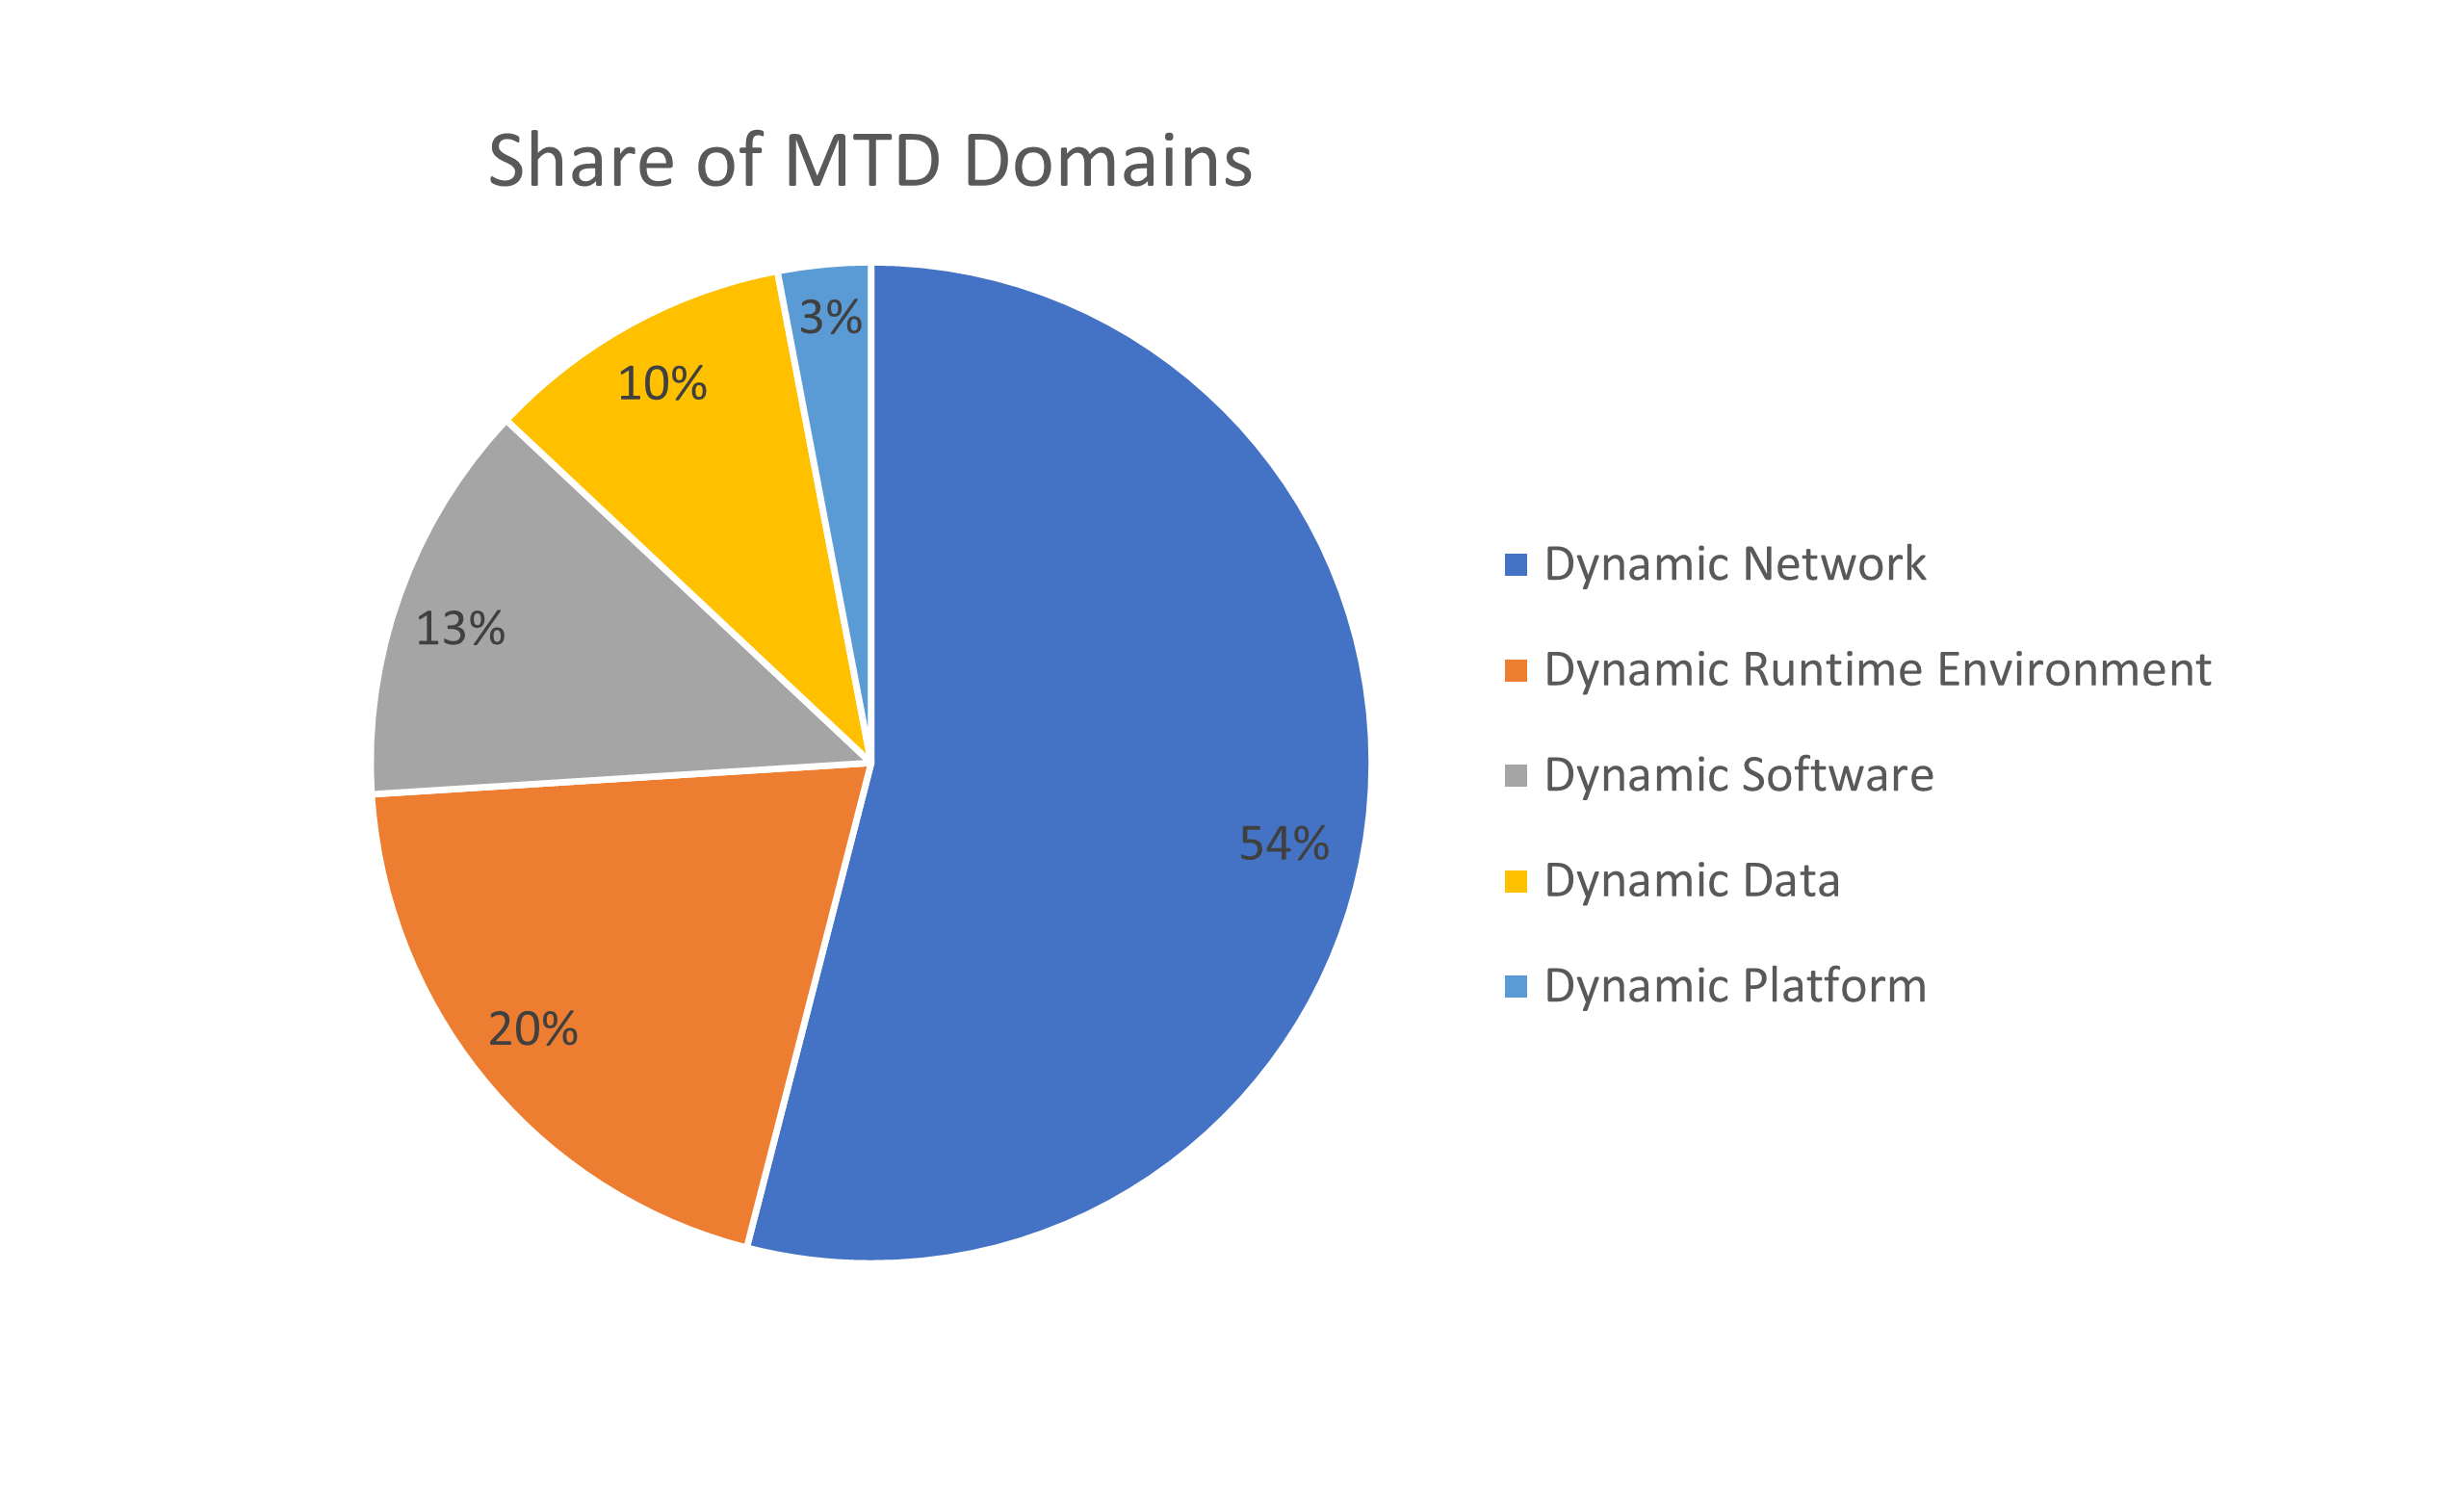
\includegraphics[scale=0.6]{assets/shareOfMTDDomains.png}
\centering
\caption{Share of IoT MTD Techniques Grouped by MTD Domains~\cite{navas:2021MTDWhere}.  }
    \label{graphic:IoTShare}
\end{figure}

The third research question was how sound the security foundations of the proposed techniques are. To answer this question, the authors classified each of the 32 techniques into three different cryptographic categories. The first category, which includes twelve techniques, completely lacks cryptography or uses a random process without providing further information about it. The second category either uses cryptographic techniques that are known to be vulnerable or uses custom cryptography without proof. Nine techniques fall into this second category. The last category is the one that has adequate security foundations, such as using state-of-the-art cryptography like SHA256. There are eleven techniques in this category. The authors point out that although they have simplified the measurement of security, 32\% is a small value considering that the central goal of MTD is to improve security. The fourth research question is the most interesting and relates to the extent to which the proposals are applicable in a real-world IoT deployment. To answer this, the implementation and evaluation aspects of the proposed techniques were examined by the authors. They concluded that 50\% of the proposed techniques show very strong or strong evidence that they can be used in a real IoT deployment. Another 25\% of the techniques show mild evidence, and another 25\% have weak to no evidence that they can be used in a real IoT deployment. The authors conclude that these are encouraging results.


\section{MTD IoT Frameworks}
\label{section:MTDFramework}
%Despite a thorough literature research, it was not possible to find any other articles on the topics of cooperative defense, IoT, and MTD. In particular, the cooperative defense part was missing, so the focus lies on articles that studied MTD and IoT in this chapter.   

\cite{article:vonderAssen} presented an MTD framework aimed at mitigating multi-purpose malware. The framework consists of two modules, the MTD decision module, which decides when to deploy an MTD mechanism, and the MTD enforcement module, which decides what MTD mechanism to deploy and how to do that. The authors distinguished between a rule-based proactive approach and a machine-learning based reactive approach to determine when the MTD mechanisms should be executed. They were able to detect normal and malicious behavior in about 10 seconds.~\cite{article:Cedeno} wrote a bachelor thesis, whose results are part of~\cite{article:vonderAssen}. This thesis is about mitigating cyberattacks on resource-constrained devices using MTD. To achieve this, the author developed an architecture consisting of three main components, an \textit{MTD Deployer Server}, an \textit{MTD Deployer Client}, and the MTD solution itself. The \textit{MTD Deployer Client} serves as an interface for external programs to notify the \textit{MTD Deployer Server} of an attack. After the \textit{MTD Deployer Server} receives an attack report, it searches for the appropriate MTD solution, whereupon the \textit{MTD Deployer Server} launches the appropriate script of the MTD solution to mitigate the attack on the affected machine. This architecture was also the basis for the thesis at hand.


\cite{article:mercado-velazquez} created a framework that helps to answer the fundamental design questions (What, How, When) described in Section \ref{section:MTD} by using five different variables: attack success probability, system downtime, CPU time, energy consumption, and memory usage. The framework starts with policies, i.e., desirable goals and targets to be achieved. Then some strategy parameters (what to move, when to move, and how to move) are defined. These parameters are then applied to the IoT system which will be continuously attacked. During these attacks, the five variables are measured. These variables are then analyzed using multiple criteria decision analysis. The result of this analysis is compared to the targets defined in the policies. Depending on this comparison, either the final strategy parameters are fixed or different strategy parameters need to be created and the framework starts over.
Finally, the authors used this framework to select the most suitable "when to move" parameter for a proposed MTD technique.


\cite{NavasDefenseFramework} proposed a generic MTD framework for IoT called IANVS. This framework consists of four different components that should facilitate the implementation of MTD in distributed systems, since in such systems the parties involved need to agree on the MP value. The four components are

\begin{itemize}
    \item An authenticated key establishment mechanism called AKE. This provides a secret cryptographic key that only trusted parties of the MTD strategy must know.  
    \item An authenticated state synchronization mechanism called Auth-SYNC. This provides a system state value that must be fresh and authenticated. 
    \item A cryptographically secure pseudo random number generator called CSPRNG. This takes the cryptographic key from the AKE component and the system state from the Auth-SYNC component and generates a "cryptographically secure pseudo random binary key stream". 
    \item A mechanism called MP-Map that outputs values in the MP domains with equiprobability. This takes the keystream from the CSPRNG and maps it to a value in the MP domain (e.g. port hopping).
\end{itemize}

The authors also applied this framework and designed two MTD techniques for IoT.



\section{MTD IoT Mechanisms}
This subsection briefly introduces MTD mechanisms/techniques. Since the intention is to use dynamic network techniques for the implementation part of this thesis, this subsection is mostly limited to this type of techniques. However, other techniques that were in the same articles as the dynamic network techniques are also briefly mentioned. 

\cite{article:MT6D} proposed "MT6D", which stands for Moving Target IPv6 defense, with the goal of protecting hosts communicating over the public Internet from targeted network attacks while preserving user privacy. To achieve this, repeated address rotation of the sender and receiver takes place. This address rotation can also occur in mid-session, preventing an attacker from knowing who the two hosts are. The MT6D IIDs are computed from a host's EUI-64 IID, a timestamp, and a shared session key. The authors ultimately validated their design with a proof-of-concept MT6D prototype. 

\cite{article:6LowPAN} further adapted this approach for IoT. The authors investigated how this MT6D can be used with the "IPv6 over Low power Wireless Personal Area Network" (6LoWPAN). The authors concluded that frequent rotation of IPv6 addresses of 6LoWPAN devices can prevent an attacker from obtaining the IP address of a device and thus prevent an attack. Further research based on MT6D was done by~\cite{article:microMovingTarget}, who presented optimizations and the design for a Micro-Moving Target IPv6 Defense (μMT6D
). This includes the protocols, the description of the operating modes, and the lightweight hash algorithms. Additionally, the authors present detailed testing and validation possibilities.


\cite{artice:defenseApproach} also proposed MTD techniques for resource-constrained devices. Their approach involves reconfiguring such devices at two different architectural layers. The first is the security layer, where the reconfiguration is performed by switching between different cryptosystems in the embedded network. The second layer is the physical layer, where the reconfiguration of the devices can be done through different versions of the firmware. The authors concluded that their proposed mechanism increases the complexity for a potential attacker.


\cite{article:addressHopping} suggested 6HOP. This algorithm provides transient addresses, ports, and key information for the connection endpoints (e.g. server and client). These endpoints must be initialized over a residential wireless network to exchange a secret. From this secret, the corresponding information is deterministically computed using the 6HOP algorithm. Thus, a server knows which address to assign to itself and on which port to listen for incoming requests, and the client knows where to connect. 


\cite{article:vonderAssen}, which was mentioned in the previous section, proposed several MTD mechanisms in addition to the MTD framework. The first mechanism is to honeypot and trap a crypto-ransomware encryptor with dynamically expanding and collapsing directories of dummy files. Along with this trapping, the encryptor is identified and killed. The second mechanism is to change the file extension of critical data to prevent it from being encrypted by crypto ransomware. This works because the file extensions determine whether or not the files are a target for some malware families. The third mechanism was to remove malware such as rootkits with a clean \textit{ld.so.preload} file. The last mechanism was to randomize private IP addresses to deal with C\&C malware, as the IP address change disrupts the communication between the IoT device and the C\&C. These MTD mechanisms were then successfully tested against real malware.


\cite{article:asha} proposed an address shuffling algorithm (AShA). The idea of this algorithm is to let each node of a network calculate its new address autonomously. A coordinator ensures that each new address is not already in use in the network by choosing a set of parameters. ASha enables secure, fast, and collision-free address renewal in an IPv6 network.  





\cite{NavasDefenseFramework} proposed two concrete MTD techniques using the framework explained above (IANVS). The first is a single port-hopping strategy using the UDP port number of a service as the moving parameter. Since known port numbers are a prerequisite for network services to work, their framework is required for port hopping while informing other parties in the network of the current port. The second strategy is to prevent DoS attacks on CoAP servers. The moving parameter here is the \textit{/.well-known/core} URI, and the idea is that the server should only respond to GET requests from clients if the encoded GET request matches the present MTD representation of \textit{/.well-known/core}. Finally, the authors evaluated the port-hopping strategy on real IoT hardware. 


\cite{article:mercado-velazquez} proposed an MTD strategy that shuffles between 4 communication protocols between a node and the gateway in the IoT network by applying their proposed framework that was presented in the previous chapter. Examples of the communication protocols are WiFi and Bluetooth. By using the framework the authors found the ideal when to move parameter for their MTD strategy. This strategy ultimately involved changing the communication protocol with an uniform random shuffling and at a uniform random time between 1.5 minutes and 2.5 minutes.


Table \ref{table:relatedWork} shows the described network techniques with some additional information. It is evident that there exist several different approaches to defend IoT against malware. However, no approach has been found that includes a cooperative component to more effectively defend against IoT malware. As there is an increasing threat caused by such malware~\cite{website:KasperskyAMalwareStory}~\cite{website:trendmicroTheFuture}, further research is needed. This thesis addresses this research gap.  



 \begin{sidewaystable}[tph]
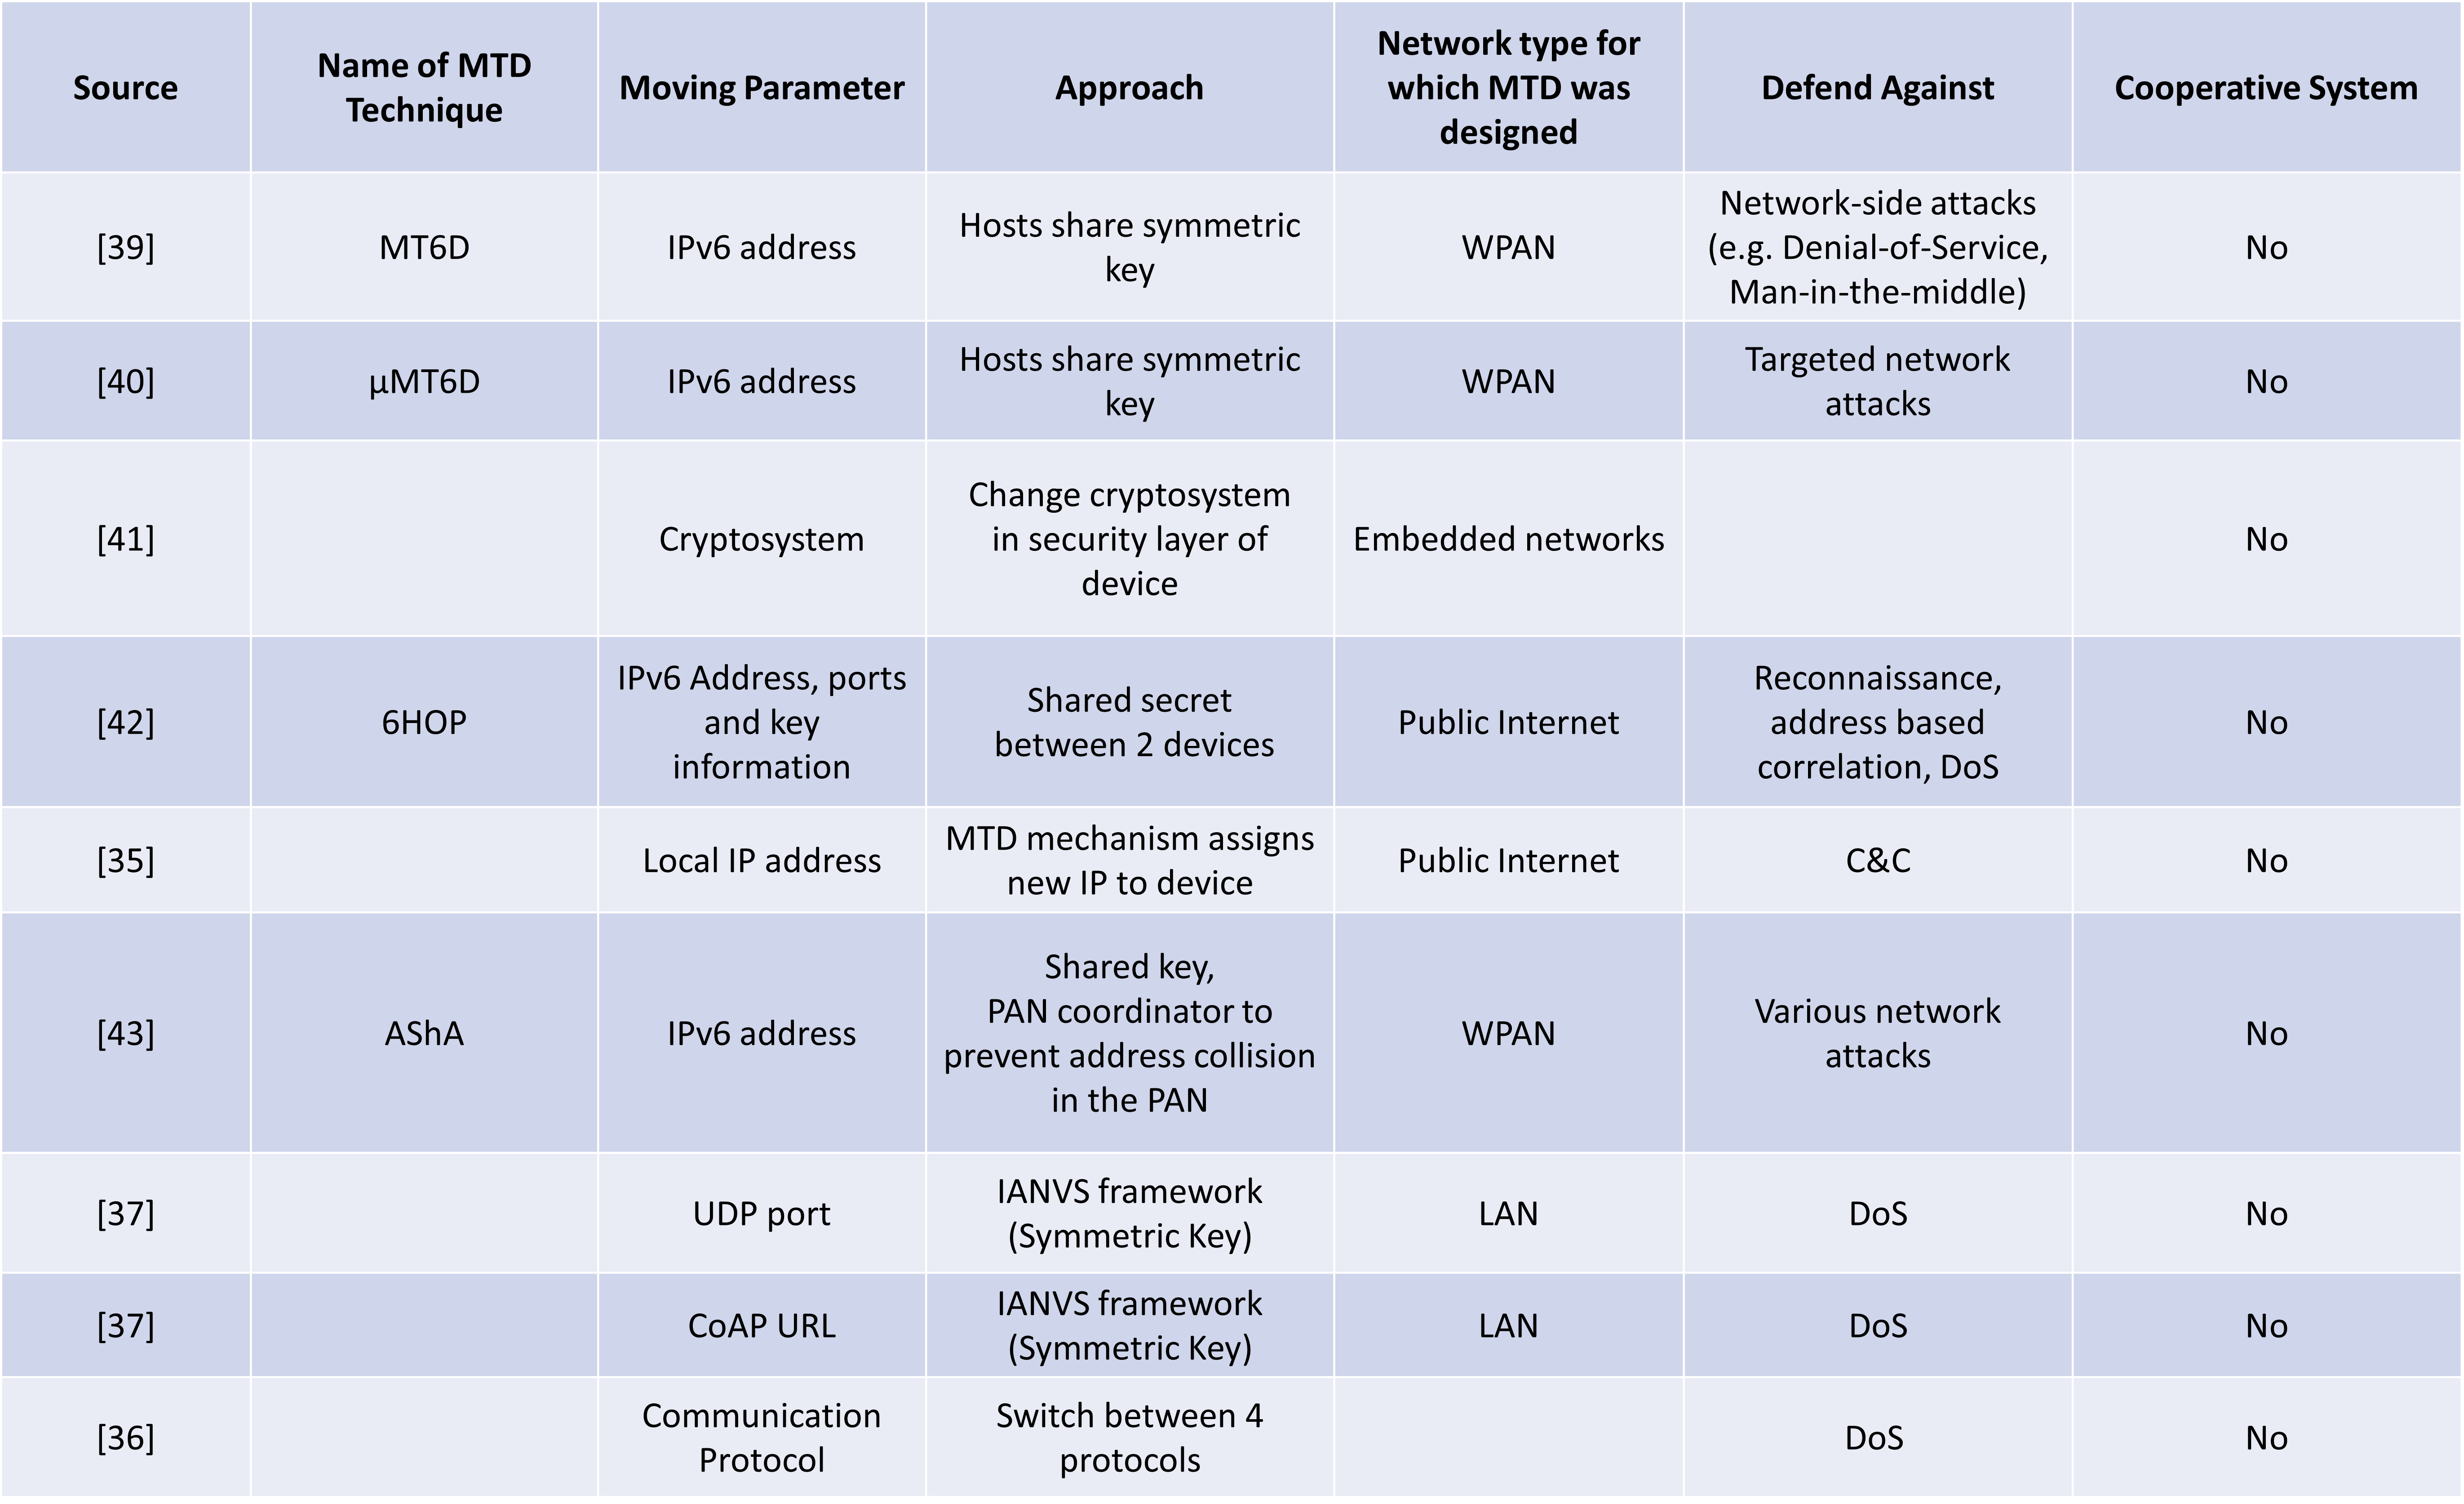
\includegraphics[scale=0.55]{assets/relatedWork.png}
\centering
\caption{A Table Summarizing Related Research.}
    \label{table:relatedWork}
\end{sidewaystable}
